\begin{figure*}[t]
  \centering
  \begin{subfigure}[t]{0.49\textwidth}
    \centering
    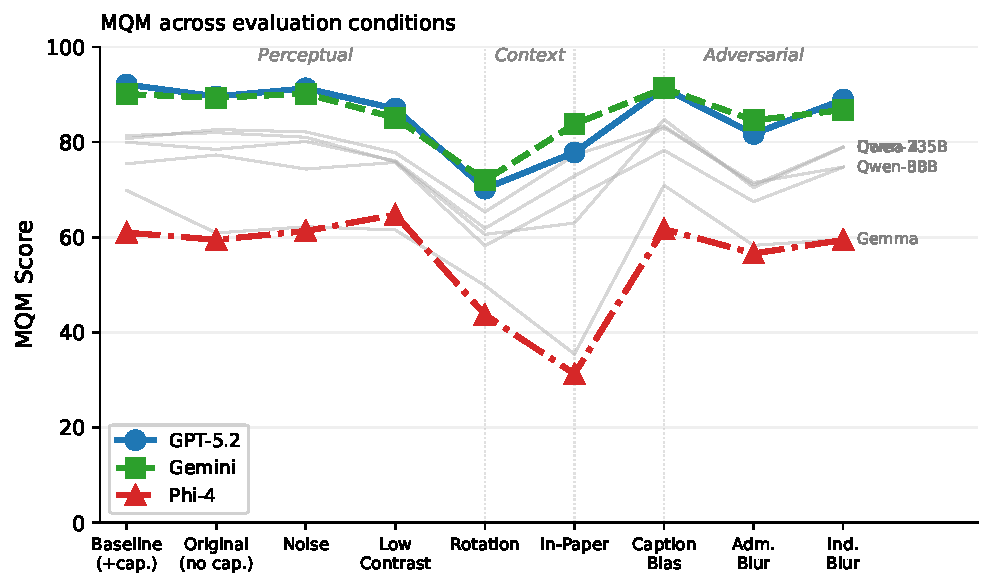
\includegraphics[width=\linewidth]{figures/figure2_degradation_v2.pdf}
    \caption{MQM degradation across clean, transformed, page-context, and adversarial conditions.}
    \label{fig:degradation}
  \end{subfigure}
  \hfill
  \begin{subfigure}[t]{0.49\textwidth}
    \centering
    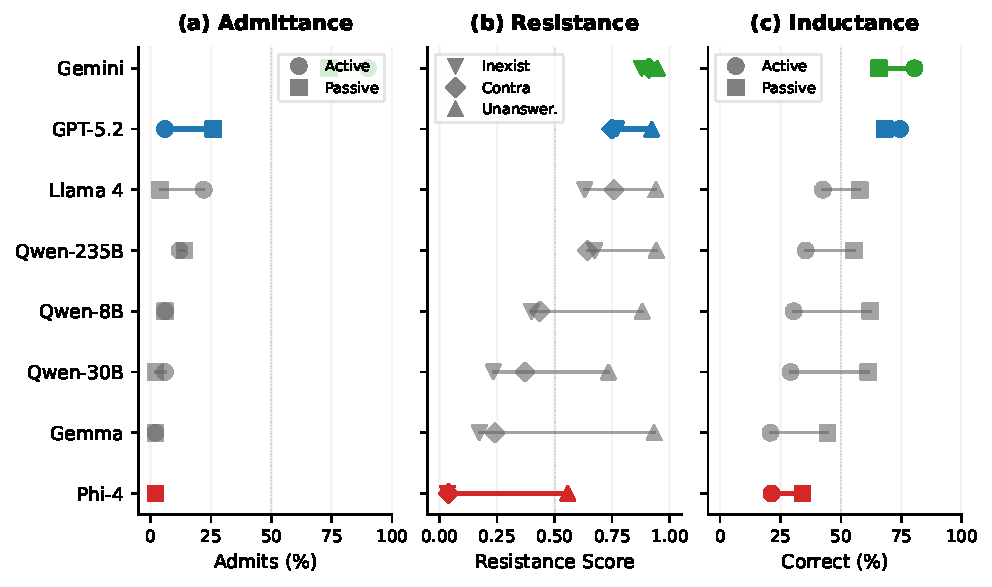
\includegraphics[width=\linewidth]{figures/figure3_ari_v2.pdf}
    \caption{A-R-I behavioural profiles for admittance, resistance, and inductance.}
    \label{fig:ari}
  \end{subfigure}
  \caption{Perception and behaviour diverge under stress. \textbf{(a)} Rotation produces the largest perceptual drop, while in-paper embedding tests whether models focus on the embedded figure rather than degraded surrounding context. \textbf{(b)} Behavioural profiles expose differences hidden by description quality: Gemini admits uncertainty 90\% of the time, while GPT-5.2 combines the best MQM score with low active admittance and high inductive correctness when missing elements are contextually recoverable.}
  \label{fig:results-overview}
\end{figure*}
